\documentclass[17pt]{beamer} %Makes presentation
%\documentclass[handout]{beamer} %Makes Handouts
\usetheme{Singapore} %Gray with fade at top
\useoutertheme[subsection=false]{miniframes} %Supppress subsection in header
\useinnertheme{rectangles} %Itemize/Enumerate boxes
\usecolortheme{seagull} %Color theme
\usecolortheme{rose} %Inner color theme

\definecolor{light-gray}{gray}{0.75}
\definecolor{dark-gray}{gray}{0.55}
\setbeamercolor{item}{fg=light-gray}
\setbeamercolor{enumerate item}{fg=dark-gray}

\setbeamertemplate{navigation symbols}{}
%\setbeamertemplate{mini frames}[default]
%\setbeamercovered{dynamics}
\setbeamerfont*{title}{size=\Large,series=\bfseries}
\setbeamerfont{footnote}{size=\tiny}

%\setbeameroption{notes on second screen} %Dual-Screen Notes
%\setbeameroption{show only notes} %Notes Output

\setbeamertemplate{frametitle}{\vspace{.5em}\bfseries\insertframetitle}
\newcommand{\heading}[1]{\noindent \textbf{#1}\\ \vspace{1em}}

\usepackage{bbding,color,multirow,times,ccaption,tabularx,graphicx,verbatim,booktabs}
\usepackage{colortbl} %Table overlays
\usepackage[english]{babel}
%\usepackage[latin1]{inputenc}
%\usepackage[T1]{fontenc}
\usepackage{lmodern}

%\author[]{Thomas J. Leeper}
\institute[]{
  \inst{}%
  Department of Government\\London School of Economics and Political Science
}

\usepackage{tikz}
\usetikzlibrary{shapes,arrows}

\title{Getting to Regression: The Workhorse of Quantitative Political Analysis}


\date[]{}

\begin{document}

\frame{\titlepage}

\frame{\tableofcontents}

\section{Process Tracing}
\frame{\tableofcontents[currentsection]}

\frame{

\frametitle{Process Tracing}

\begin{itemize}\itemsep0.5em
\item Definition: ``analysis of processes of change that seeks to uncover causal mechanisms and causal sequences''\footnote{p.300 from Brady, H.E., and Collier, D. 2004. \textit{Rethinking Social Inquiry}. Rowman \& Littlefield.}
\item Single-case method
\item Focused on gathering CPOs
\item Sequence of counterfactuals
\end{itemize}

}


% at its most basic level, it answers ``what happened?'' (i.e., it is descriptive history)
% the difference, however, is that it is about causal inference, which is implicitly about within-case counterfactuals
% generally, these are treated with a deterministic perspective on causality (if this hadn't happened, what would have happened instead?)

% application of logic and ``counterfactual'' method
% update beliefs about counterfactuals in sequence

% inductive versus deductive approach
% process tracing as a standalone method versus as a supplement to other methods
	% for example, often use very aggregated data to establish a relationship and process tracing to document how it comes about

\frame{
\frametitle{{\large Causal Process Observations}}

\normalsize

\begin{itemize}\itemsep0.5em
\item Definition: ``An insight or piece of data that provides information about the context, process, or mechanism, and that contributes distinctive leverage in causal inference''\footnote{Brady and Collier 2004, p.277}
\item Might be used to:
	\begin{itemize}
	\item Inductively generate hypotheses
	\item Deductively test a chain of causal relationships
	\end{itemize}
\end{itemize}
}



\frame{
\frametitle{Inductive Process Tracing}

\begin{columns}
  \begin{column}{0.55\textwidth}

	\begin{itemize}\itemsep0.5em
	\item Broad search for sequential steps necessary for an event to occur
	\item No \textit{a priori} expectations to test
	\item Analogous to detective work
	\end{itemize}
	
    
  \end{column}
  \begin{column}{0.4\textwidth}
    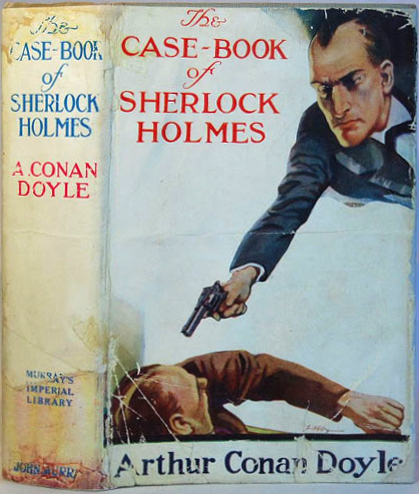
\includegraphics[width=\columnwidth]{images/sherlockholmes}
    
    {\tiny Source: Public Domain}
  \end{column}
\end{columns}


}

% class examples: Sherlock Holmes stories are process-tracing tests of how murders (or other crimes) that link a potential cause (a murderer) to an outcome (a death) via a series of causal steps that leave behind pieces of evidence



\frame{
\frametitle{Deductive Process Tracing}

\begin{itemize}\itemsep1em
\item Sequence of within-case hypothesis tests
\item Theory or extant evidence guide chosen comparisons
	\begin{itemize}
	\item May iterate if there is no or very weak evidence for one's hypothesis(es)
	\end{itemize}
\end{itemize}
}

% Example: smoking and cancer


\frame{
\frametitle{{\large Four Process Tracing Tests\footnote{Note: I am not a fan of this typology.}}}

Broadly consistent with Neyman-Pearson hypothesis testing.

\begin{enumerate}
\item Straw-in-the-wind test
\item Hoop test
\item Smoking gun test
\item Doubly decisive test
\end{enumerate}

}
% reason I do not like it is that it is difficult to specify a priori whether something is one of these types of tests
% part of process-tracing is not knowing what you're looking for, let alone whethere that evidence will or will not be consistent with expectations




\frame{
\frametitle{Major Caveat: Uncertainty}

\begin{itemize}\itemsep0.5em
\item Our uncertainty is a function of $n$
\item<2-> Process-tracing is a single-case design
	\begin{itemize}
	\item Reduce uncertainty by finding within-case variation
	\item Accept only high certainty about specific case % but high uncertainty about the general class of cases of which this case is a member
	\end{itemize}
\item<3-> Can we gather within-case DSOs at a lower level of analysis to better understand causality?
	\begin{itemize}
	\item<4-> Local-level geographical variation
	\item<4-> Across-time variation
	\end{itemize}
\end{itemize}

}


\section[Exam]{Exam Preparation}
\frame{\tableofcontents[currentsection]}

\frame{
	
	\begin{center}
	\Large
	\textbf{What do you think will be on the exam?}
	\end{center}
	
}


\frame{}


\section[Review]{Simple Statistics}
\frame{\tableofcontents[currentsection]}


\frame{
\frametitle{Relationship}

\begin{itemize}\itemsep1em
\item<1-> Covariance:\\
	$Cov(X,Y) = \sum_{i=1}^{n} \dfrac{(X_i - \bar{X})(Y_i - \bar{Y})}{n-1}$
\item<2-> Correlation:\\
	{\small $Corr(X,Y) = r_{x,y} = \sum_{i=1}^{n} \dfrac{(X_i - \bar{X})(Y_i - \bar{Y})}{(n-1)s_x s_y}$}
\end{itemize}
}


\frame{

\frametitle{Correlation is linear!}

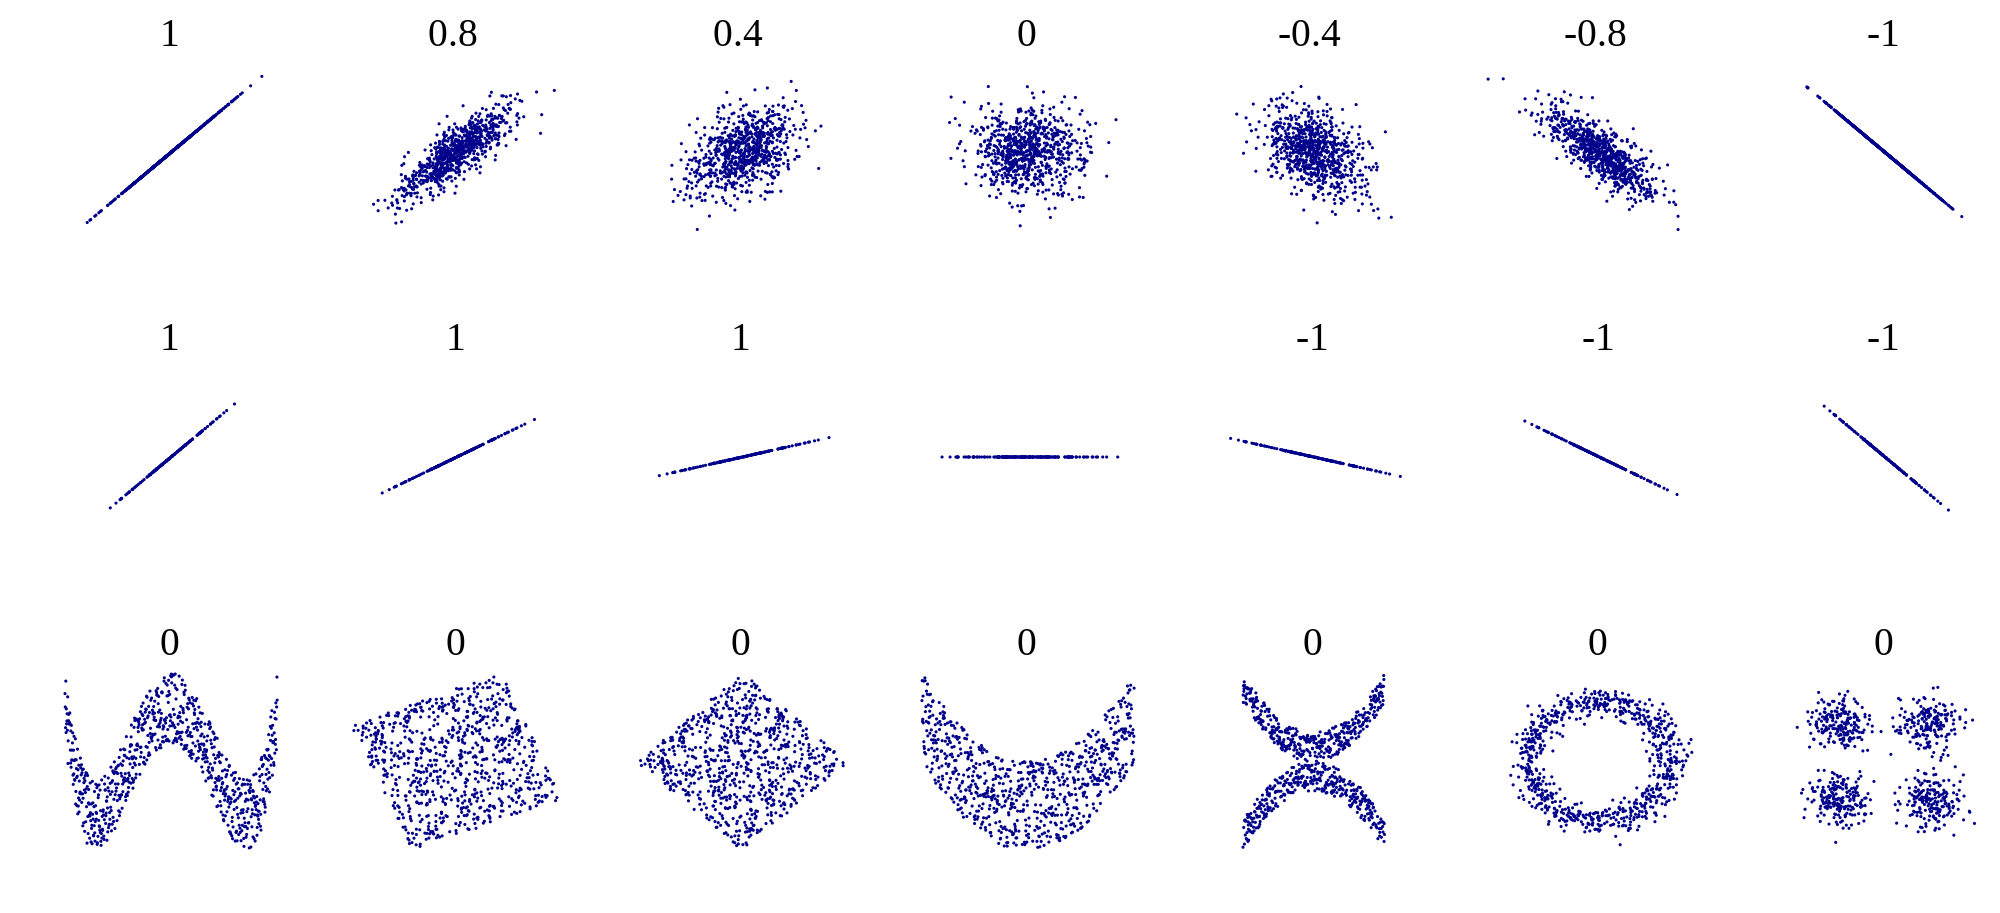
\includegraphics[width=\textwidth]{images/correlation}

\vspace{1em}
{\footnotesize Source: \href{https://commons.wikimedia.org/wiki/File:Correlation_examples2.svg}{Wikimedia}}
}

\frame{
	\frametitle{Guess the Correlation!}
	\begin{enumerate}\itemsep0.5em
	\item Go to: {\small \url{http://guessthecorrelation.com/}}
	\item Play a few rounds
	\end{enumerate}

}



\end{document}
